\documentclass[a4paper]{book}
\usepackage{a4wide}
\usepackage{makeidx}
\usepackage{graphicx}
\usepackage{multicol}
\usepackage{float}
\usepackage{listings}
\usepackage{color}
\usepackage{textcomp}
\usepackage{alltt}
\usepackage{times}
\usepackage{ifpdf}
\ifpdf
\usepackage[pdftex,
            pagebackref=true,
            colorlinks=true,
            linkcolor=blue,
            unicode
           ]{hyperref}
\else
\usepackage[ps2pdf,
            pagebackref=true,
            colorlinks=true,
            linkcolor=blue,
            unicode
           ]{hyperref}
\usepackage{pspicture}
\fi
\usepackage[utf8]{inputenc}
\usepackage{doxygen}
\lstset{language=C++,inputencoding=utf8,basicstyle=\footnotesize,breaklines=true,breakatwhitespace=true,tabsize=8,numbers=left }
\makeindex
\setcounter{tocdepth}{3}
\renewcommand{\footrulewidth}{0.4pt}
\begin{document}
\hypersetup{pageanchor=false}
\begin{titlepage}
\vspace*{7cm}
\begin{center}
{\Large Solomon \\[1ex]\large 1.0 (Build 52) }\\
\vspace*{1cm}
{\large Generated by Doxygen 1.6.2}\\
\vspace*{0.5cm}
{\small Mon Mar 1 03:58:59 2010}\\
\end{center}
\end{titlepage}
\clearemptydoublepage
\pagenumbering{roman}
\tableofcontents
\clearemptydoublepage
\pagenumbering{arabic}
\hypersetup{pageanchor=true}
\chapter{Class Index}
\section{Class Hierarchy}
This inheritance list is sorted roughly, but not completely, alphabetically:\begin{DoxyCompactList}
\item \contentsline{section}{itc.AI}{\pageref{classitc_1_1_a_i}}{}
\item \contentsline{section}{itc.CTactic}{\pageref{classitc_1_1_c_tactic}}{}
\begin{DoxyCompactList}
\item \contentsline{section}{itc.tactic.CTactic\_\-a0}{\pageref{classitc_1_1tactic_1_1_c_tactic__a0}}{}
\item \contentsline{section}{itc.tactic.CTactic\_\-a1}{\pageref{classitc_1_1tactic_1_1_c_tactic__a1}}{}
\item \contentsline{section}{itc.tactic.CTactic\_\-a2}{\pageref{classitc_1_1tactic_1_1_c_tactic__a2}}{}
\item \contentsline{section}{itc.tactic.CTactic\_\-d0}{\pageref{classitc_1_1tactic_1_1_c_tactic__d0}}{}
\item \contentsline{section}{itc.tactic.CTactic\_\-ea0}{\pageref{classitc_1_1tactic_1_1_c_tactic__ea0}}{}
\item \contentsline{section}{itc.tactic.CTactic\_\-ea1}{\pageref{classitc_1_1tactic_1_1_c_tactic__ea1}}{}
\item \contentsline{section}{itc.tactic.CTactic\_\-ed0}{\pageref{classitc_1_1tactic_1_1_c_tactic__ed0}}{}
\end{DoxyCompactList}
\item \contentsline{section}{itc.solomon}{\pageref{classitc_1_1solomon}}{}
\end{DoxyCompactList}

\chapter{Class Index}
\section{Class List}
Here are the classes, structs, unions and interfaces with brief descriptions:\begin{DoxyCompactList}
\item\contentsline{section}{\hyperlink{classitc_1_1_a_i}{itc.AI} }{\pageref{classitc_1_1_a_i}}{}
\item\contentsline{section}{\hyperlink{classitc_1_1_c_tactic}{itc.CTactic} }{\pageref{classitc_1_1_c_tactic}}{}
\item\contentsline{section}{\hyperlink{classitc_1_1tactic_1_1_c_tactic__a0}{itc.tactic.CTactic\_\-a0} }{\pageref{classitc_1_1tactic_1_1_c_tactic__a0}}{}
\item\contentsline{section}{\hyperlink{classitc_1_1tactic_1_1_c_tactic__a1}{itc.tactic.CTactic\_\-a1} }{\pageref{classitc_1_1tactic_1_1_c_tactic__a1}}{}
\item\contentsline{section}{\hyperlink{classitc_1_1tactic_1_1_c_tactic__a2}{itc.tactic.CTactic\_\-a2} }{\pageref{classitc_1_1tactic_1_1_c_tactic__a2}}{}
\item\contentsline{section}{\hyperlink{classitc_1_1tactic_1_1_c_tactic__d0}{itc.tactic.CTactic\_\-d0} }{\pageref{classitc_1_1tactic_1_1_c_tactic__d0}}{}
\item\contentsline{section}{\hyperlink{classitc_1_1tactic_1_1_c_tactic__ea0}{itc.tactic.CTactic\_\-ea0} }{\pageref{classitc_1_1tactic_1_1_c_tactic__ea0}}{}
\item\contentsline{section}{\hyperlink{classitc_1_1tactic_1_1_c_tactic__ea1}{itc.tactic.CTactic\_\-ea1} }{\pageref{classitc_1_1tactic_1_1_c_tactic__ea1}}{}
\item\contentsline{section}{\hyperlink{classitc_1_1tactic_1_1_c_tactic__ed0}{itc.tactic.CTactic\_\-ed0} }{\pageref{classitc_1_1tactic_1_1_c_tactic__ed0}}{}
\item\contentsline{section}{\hyperlink{classitc_1_1solomon}{itc.solomon} }{\pageref{classitc_1_1solomon}}{}
\end{DoxyCompactList}

\chapter{Class Documentation}
\hypertarget{classitc_1_1_a_i}{
\section{itc.AI Class Reference}
\label{classitc_1_1_a_i}\index{itc::AI@{itc::AI}}
}
\subsection*{Static Public Member Functions}
\begin{DoxyCompactItemize}
\item 
\hypertarget{classitc_1_1_a_i_a4f6a76cbca96e226d6045caa79180bbb}{
static byte {\bfseries getGaugingThreshold} ()}
\label{classitc_1_1_a_i_a4f6a76cbca96e226d6045caa79180bbb}

\item 
\hypertarget{classitc_1_1_a_i_a7fd6d93d400c4b5887de390dbb8b7117}{
static void {\bfseries setGaugingThreshold} (byte \hyperlink{classitc_1_1_a_i_a55e666c1cfd457046c1b2ddfc2b44d62}{gaugingThreshold})}
\label{classitc_1_1_a_i_a7fd6d93d400c4b5887de390dbb8b7117}

\item 
static int \hyperlink{classitc_1_1_a_i_ad9fb9145c1561f60c2011ad877ea8a0a}{pickTactic} (int status, int currentTacticIndex, \hyperlink{classitc_1_1_c_tactic}{CTactic} tacticLibrary\mbox{[}$\,$\mbox{]}\mbox{[}$\,$\mbox{]})
\item 
static byte \hyperlink{classitc_1_1_a_i_a8cf895fa4d48d6f2c6f17bd49d46ffaa}{gaugeTactic} (double healthBefore, double currentHealth)
\end{DoxyCompactItemize}
\subsection*{Static Public Attributes}
\begin{DoxyCompactItemize}
\item 
static byte \hyperlink{classitc_1_1_a_i_a55e666c1cfd457046c1b2ddfc2b44d62}{gaugingThreshold} = 3
\end{DoxyCompactItemize}


\subsection{Detailed Description}
This class is Solomon's decision making component. Here it assesses the past experiences and judges whether the tactic was successful in the past. \begin{DoxyAuthor}{Author}
Ciaran McCann 
\end{DoxyAuthor}


\subsection{Member Function Documentation}
\hypertarget{classitc_1_1_a_i_a8cf895fa4d48d6f2c6f17bd49d46ffaa}{
\index{itc::AI@{itc::AI}!gaugeTactic@{gaugeTactic}}
\index{gaugeTactic@{gaugeTactic}!itc::AI@{itc::AI}}
\subsubsection[{gaugeTactic}]{\setlength{\rightskip}{0pt plus 5cm}static byte itc.AI.gaugeTactic (double {\em healthBefore}, \/  double {\em currentHealth})\hspace{0.3cm}{\ttfamily  \mbox{[}static\mbox{]}}}}
\label{classitc_1_1_a_i_a8cf895fa4d48d6f2c6f17bd49d46ffaa}
Returns a one or a zero based on the health change in the time before a tactic was used and after to determine if it's a successful tactic 
\begin{DoxyParams}{Parameters}
\item[{\em healthBefore}]\item[{\em currentHealth}]\end{DoxyParams}
\begin{DoxyReturn}{Returns}

\end{DoxyReturn}
\hypertarget{classitc_1_1_a_i_ad9fb9145c1561f60c2011ad877ea8a0a}{
\index{itc::AI@{itc::AI}!pickTactic@{pickTactic}}
\index{pickTactic@{pickTactic}!itc::AI@{itc::AI}}
\subsubsection[{pickTactic}]{\setlength{\rightskip}{0pt plus 5cm}static int itc.AI.pickTactic (int {\em status}, \/  int {\em currentTacticIndex}, \/  {\bf CTactic} {\em tacticLibrary}\mbox{[}$\,$\mbox{]}\mbox{[}$\,$\mbox{]})\hspace{0.3cm}{\ttfamily  \mbox{[}static\mbox{]}}}}
\label{classitc_1_1_a_i_ad9fb9145c1561f60c2011ad877ea8a0a}
Picks a tactic for the robot based on the current status it's in i.e defensive, aggressive etc. It then calls another method isGoodTactic() which will find if the tactic as been successful in the past 
\begin{DoxyParams}{Parameters}
\item[{\em status}]\item[{\em currentTacticIndex}]\item[{\em tacticLibrary}]\end{DoxyParams}
\begin{DoxyReturn}{Returns}
Tactic to be used 
\end{DoxyReturn}


\subsection{Member Data Documentation}
\hypertarget{classitc_1_1_a_i_a55e666c1cfd457046c1b2ddfc2b44d62}{
\index{itc::AI@{itc::AI}!gaugingThreshold@{gaugingThreshold}}
\index{gaugingThreshold@{gaugingThreshold}!itc::AI@{itc::AI}}
\subsubsection[{gaugingThreshold}]{\setlength{\rightskip}{0pt plus 5cm}byte {\bf itc.AI.gaugingThreshold} = 3\hspace{0.3cm}{\ttfamily  \mbox{[}static\mbox{]}}}}
\label{classitc_1_1_a_i_a55e666c1cfd457046c1b2ddfc2b44d62}
This is the percentage amount of negative change which is required or greater to get a negative result on the efficiency 

The documentation for this class was generated from the following file:\begin{DoxyCompactItemize}
\item 
/Users/carllange/Documents/workspace/Solomon/src/itc/AI.java\end{DoxyCompactItemize}

\hypertarget{classitc_1_1_c_tactic}{
\section{itc.CTactic Class Reference}
\label{classitc_1_1_c_tactic}\index{itc::CTactic@{itc::CTactic}}
}
Inheritance diagram for itc.CTactic::\begin{figure}[H]
\begin{center}
\leavevmode
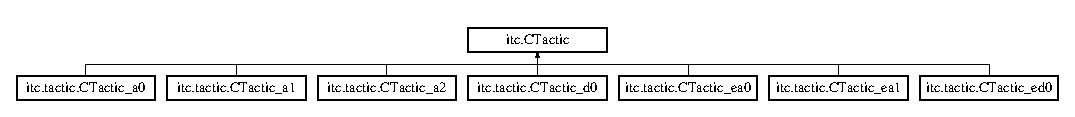
\includegraphics[height=1.12676cm]{classitc_1_1_c_tactic}
\end{center}
\end{figure}
\subsection*{Public Member Functions}
\begin{DoxyCompactItemize}
\item 
void \hyperlink{classitc_1_1_c_tactic_ae5f5c51a6e04d22bc298dbdec4080770}{run\_\-} (\hyperlink{classitc_1_1solomon}{solomon} s)
\item 
void \hyperlink{classitc_1_1_c_tactic_a63a5a64ff30293061e37eca71fb77a96}{onScannedRobot\_\-} (\hyperlink{classitc_1_1solomon}{solomon} s, ScannedRobotEvent e)
\item 
void \hyperlink{classitc_1_1_c_tactic_a9a8d125f826667459758f2767c3bd957}{onHitByBullet\_\-} (\hyperlink{classitc_1_1solomon}{solomon} s, HitByBulletEvent e)
\item 
void \hyperlink{classitc_1_1_c_tactic_a19cf73207948eff2c6db7d90fce8bd55}{onHitRobot\_\-} (\hyperlink{classitc_1_1solomon}{solomon} s, HitRobotEvent e)
\item 
boolean \hyperlink{classitc_1_1_c_tactic_aefcf5f13687e17eaa8bf5dd4be3b424b}{isGoodTactic} (int status)
\end{DoxyCompactItemize}
\subsection*{Protected Member Functions}
\begin{DoxyCompactItemize}
\item 
void \hyperlink{classitc_1_1_c_tactic_a3d4f7c60b5eb048608b96e4c8c8fad24}{fire} (\hyperlink{classitc_1_1solomon}{solomon} s, double enemyDist)
\item 
double \hyperlink{classitc_1_1_c_tactic_ae1e7b81085c04b6d03be93dfefec5b0f}{getRandom} ()
\item 
double \hyperlink{classitc_1_1_c_tactic_a89a1395008161bfeed448b60a4addc7d}{getRandom} (int highest)
\item 
void \hyperlink{classitc_1_1_c_tactic_aadc353c46b7efae5844a1803dff12ce7}{turnGunRightRadians} (\hyperlink{classitc_1_1solomon}{solomon} s, double amountToRotateRadians)
\item 
void \hyperlink{classitc_1_1_c_tactic_a93bd30da3b2689b475ab0bdc9220ae77}{turnRadarRightRadians} (\hyperlink{classitc_1_1solomon}{solomon} s, double amountToRotateRadians)
\item 
void \hyperlink{classitc_1_1_c_tactic_a6ec9c0ec24314d590adbd737bbf8be35}{turnRightRadians} (\hyperlink{classitc_1_1solomon}{solomon} s, double amountToRotateRadians)
\item 
double \hyperlink{classitc_1_1_c_tactic_a8f926b64924184c4dab8a3c5efa5d410}{getHeadingRadians} (\hyperlink{classitc_1_1solomon}{solomon} s)
\item 
double \hyperlink{classitc_1_1_c_tactic_a3218f6ba011510c64b12d87bed7adfcb}{getGunHeadingRadians} (\hyperlink{classitc_1_1solomon}{solomon} s)
\item 
double \hyperlink{classitc_1_1_c_tactic_a4d8a555f548ee605c6d67de1e262b455}{getRadarHeadingRadians} (\hyperlink{classitc_1_1solomon}{solomon} s)
\item 
double \hyperlink{classitc_1_1_c_tactic_a0fb7344f1a8072b2f764f7b76444b89e}{convertToRadians} (double degrees)
\item 
double \hyperlink{classitc_1_1_c_tactic_a89700cf4d890854f0c310a82e8f4fb8d}{convertToDegrees} (double radians)
\end{DoxyCompactItemize}
\subsection*{Protected Attributes}
\begin{DoxyCompactItemize}
\item 
\hypertarget{classitc_1_1_c_tactic_a2d99e5b6935acf7476934fac845716d6}{
final double {\bfseries GAUGING\_\-THRESHOLD} = 0.7}
\label{classitc_1_1_c_tactic_a2d99e5b6935acf7476934fac845716d6}

\item 
\hypertarget{classitc_1_1_c_tactic_a1b6717d9d6b74ce9f1d3f8e8fb18adca}{
List$<$ Byte $>$ {\bfseries gaugingList} = new ArrayList$<$Byte$>$()}
\label{classitc_1_1_c_tactic_a1b6717d9d6b74ce9f1d3f8e8fb18adca}

\item 
\hypertarget{classitc_1_1_c_tactic_a1b977fc5aa7714e83dd93c04461c5770}{
Random {\bfseries r} = new Random()}
\label{classitc_1_1_c_tactic_a1b977fc5aa7714e83dd93c04461c5770}

\end{DoxyCompactItemize}


\subsection{Member Function Documentation}
\hypertarget{classitc_1_1_c_tactic_a89700cf4d890854f0c310a82e8f4fb8d}{
\index{itc::CTactic@{itc::CTactic}!convertToDegrees@{convertToDegrees}}
\index{convertToDegrees@{convertToDegrees}!itc::CTactic@{itc::CTactic}}
\subsubsection[{convertToDegrees}]{\setlength{\rightskip}{0pt plus 5cm}double itc.CTactic.convertToDegrees (double {\em radians})\hspace{0.3cm}{\ttfamily  \mbox{[}protected\mbox{]}}}}
\label{classitc_1_1_c_tactic_a89700cf4d890854f0c310a82e8f4fb8d}
Takes in radians and converts to degrees. 
\begin{DoxyParams}{Parameters}
\item[{\em radians}]\end{DoxyParams}
\begin{DoxyReturn}{Returns}

\end{DoxyReturn}
\hypertarget{classitc_1_1_c_tactic_a0fb7344f1a8072b2f764f7b76444b89e}{
\index{itc::CTactic@{itc::CTactic}!convertToRadians@{convertToRadians}}
\index{convertToRadians@{convertToRadians}!itc::CTactic@{itc::CTactic}}
\subsubsection[{convertToRadians}]{\setlength{\rightskip}{0pt plus 5cm}double itc.CTactic.convertToRadians (double {\em degrees})\hspace{0.3cm}{\ttfamily  \mbox{[}protected\mbox{]}}}}
\label{classitc_1_1_c_tactic_a0fb7344f1a8072b2f764f7b76444b89e}
Takes in amount in degrees and returns it in radians 
\begin{DoxyParams}{Parameters}
\item[{\em degrees}]\end{DoxyParams}
\begin{DoxyReturn}{Returns}

\end{DoxyReturn}
\hypertarget{classitc_1_1_c_tactic_a3d4f7c60b5eb048608b96e4c8c8fad24}{
\index{itc::CTactic@{itc::CTactic}!fire@{fire}}
\index{fire@{fire}!itc::CTactic@{itc::CTactic}}
\subsubsection[{fire}]{\setlength{\rightskip}{0pt plus 5cm}void itc.CTactic.fire ({\bf solomon} {\em s}, \/  double {\em enemyDist})\hspace{0.3cm}{\ttfamily  \mbox{[}protected\mbox{]}}}}
\label{classitc_1_1_c_tactic_a3d4f7c60b5eb048608b96e4c8c8fad24}
Uses the distance of the enemy robot to figure out how much energy to expend when firing. The bias varies, depending on the robot's status. If it's very aggressive, it'll be more likely to fire with full strength. If very defensive, it'll almost never do that, and so on, so forth.


\begin{DoxyParams}{Parameters}
\item[{\em s}]\item[{\em enemyDist}]\end{DoxyParams}
\hypertarget{classitc_1_1_c_tactic_a3218f6ba011510c64b12d87bed7adfcb}{
\index{itc::CTactic@{itc::CTactic}!getGunHeadingRadians@{getGunHeadingRadians}}
\index{getGunHeadingRadians@{getGunHeadingRadians}!itc::CTactic@{itc::CTactic}}
\subsubsection[{getGunHeadingRadians}]{\setlength{\rightskip}{0pt plus 5cm}double itc.CTactic.getGunHeadingRadians ({\bf solomon} {\em s})\hspace{0.3cm}{\ttfamily  \mbox{[}protected\mbox{]}}}}
\label{classitc_1_1_c_tactic_a3218f6ba011510c64b12d87bed7adfcb}
Gets the gun heading in radians. 
\begin{DoxyParams}{Parameters}
\item[{\em s}]\end{DoxyParams}
\begin{DoxyReturn}{Returns}

\end{DoxyReturn}
\hypertarget{classitc_1_1_c_tactic_a8f926b64924184c4dab8a3c5efa5d410}{
\index{itc::CTactic@{itc::CTactic}!getHeadingRadians@{getHeadingRadians}}
\index{getHeadingRadians@{getHeadingRadians}!itc::CTactic@{itc::CTactic}}
\subsubsection[{getHeadingRadians}]{\setlength{\rightskip}{0pt plus 5cm}double itc.CTactic.getHeadingRadians ({\bf solomon} {\em s})\hspace{0.3cm}{\ttfamily  \mbox{[}protected\mbox{]}}}}
\label{classitc_1_1_c_tactic_a8f926b64924184c4dab8a3c5efa5d410}
Gets the heading in radians. 
\begin{DoxyParams}{Parameters}
\item[{\em s}]\end{DoxyParams}
\begin{DoxyReturn}{Returns}

\end{DoxyReturn}
\hypertarget{classitc_1_1_c_tactic_a4d8a555f548ee605c6d67de1e262b455}{
\index{itc::CTactic@{itc::CTactic}!getRadarHeadingRadians@{getRadarHeadingRadians}}
\index{getRadarHeadingRadians@{getRadarHeadingRadians}!itc::CTactic@{itc::CTactic}}
\subsubsection[{getRadarHeadingRadians}]{\setlength{\rightskip}{0pt plus 5cm}double itc.CTactic.getRadarHeadingRadians ({\bf solomon} {\em s})\hspace{0.3cm}{\ttfamily  \mbox{[}protected\mbox{]}}}}
\label{classitc_1_1_c_tactic_a4d8a555f548ee605c6d67de1e262b455}
Gets the radar heading in radians. 
\begin{DoxyParams}{Parameters}
\item[{\em s}]\end{DoxyParams}
\begin{DoxyReturn}{Returns}

\end{DoxyReturn}
\hypertarget{classitc_1_1_c_tactic_a89a1395008161bfeed448b60a4addc7d}{
\index{itc::CTactic@{itc::CTactic}!getRandom@{getRandom}}
\index{getRandom@{getRandom}!itc::CTactic@{itc::CTactic}}
\subsubsection[{getRandom}]{\setlength{\rightskip}{0pt plus 5cm}double itc.CTactic.getRandom (int {\em highest})\hspace{0.3cm}{\ttfamily  \mbox{[}protected\mbox{]}}}}
\label{classitc_1_1_c_tactic_a89a1395008161bfeed448b60a4addc7d}
Returns a number, between zero and input. 
\begin{DoxyParams}{Parameters}
\item[{\em highest}]\end{DoxyParams}
\begin{DoxyReturn}{Returns}

\end{DoxyReturn}
\hypertarget{classitc_1_1_c_tactic_ae1e7b81085c04b6d03be93dfefec5b0f}{
\index{itc::CTactic@{itc::CTactic}!getRandom@{getRandom}}
\index{getRandom@{getRandom}!itc::CTactic@{itc::CTactic}}
\subsubsection[{getRandom}]{\setlength{\rightskip}{0pt plus 5cm}double itc.CTactic.getRandom ()\hspace{0.3cm}{\ttfamily  \mbox{[}protected\mbox{]}}}}
\label{classitc_1_1_c_tactic_ae1e7b81085c04b6d03be93dfefec5b0f}
Returns a random number. \begin{DoxyReturn}{Returns}

\end{DoxyReturn}
\hypertarget{classitc_1_1_c_tactic_aefcf5f13687e17eaa8bf5dd4be3b424b}{
\index{itc::CTactic@{itc::CTactic}!isGoodTactic@{isGoodTactic}}
\index{isGoodTactic@{isGoodTactic}!itc::CTactic@{itc::CTactic}}
\subsubsection[{isGoodTactic}]{\setlength{\rightskip}{0pt plus 5cm}boolean itc.CTactic.isGoodTactic (int {\em status})}}
\label{classitc_1_1_c_tactic_aefcf5f13687e17eaa8bf5dd4be3b424b}
Calculates the efficiency of the tactic using the gaugingList and returns true or false \begin{DoxyReturn}{Returns}

\end{DoxyReturn}
\hypertarget{classitc_1_1_c_tactic_a9a8d125f826667459758f2767c3bd957}{
\index{itc::CTactic@{itc::CTactic}!onHitByBullet\_\-@{onHitByBullet\_\-}}
\index{onHitByBullet\_\-@{onHitByBullet\_\-}!itc::CTactic@{itc::CTactic}}
\subsubsection[{onHitByBullet\_\-}]{\setlength{\rightskip}{0pt plus 5cm}void itc.CTactic.onHitByBullet\_\- ({\bf solomon} {\em s}, \/  HitByBulletEvent {\em e})}}
\label{classitc_1_1_c_tactic_a9a8d125f826667459758f2767c3bd957}
This should be overwritten by every tactic. 
\begin{DoxyParams}{Parameters}
\item[{\em s}]\item[{\em e}]\end{DoxyParams}


Reimplemented in \hyperlink{classitc_1_1tactic_1_1_c_tactic__a0_a8911e3200cb13cfab22082c0a718c0b9}{itc.tactic.CTactic\_\-a0}, \hyperlink{classitc_1_1tactic_1_1_c_tactic__a2_a774862588c2b010b16e2709d922db24d}{itc.tactic.CTactic\_\-a2}, \hyperlink{classitc_1_1tactic_1_1_c_tactic__d0_a4af101273ae2df9ee3c58641e1b1e422}{itc.tactic.CTactic\_\-d0}, \hyperlink{classitc_1_1tactic_1_1_c_tactic__ea0_a66859754a34c07f83a114509a86914cb}{itc.tactic.CTactic\_\-ea0}, and \hyperlink{classitc_1_1tactic_1_1_c_tactic__ed0_ad04cdcbec1998d1c7bee55a9dc959505}{itc.tactic.CTactic\_\-ed0}.\hypertarget{classitc_1_1_c_tactic_a19cf73207948eff2c6db7d90fce8bd55}{
\index{itc::CTactic@{itc::CTactic}!onHitRobot\_\-@{onHitRobot\_\-}}
\index{onHitRobot\_\-@{onHitRobot\_\-}!itc::CTactic@{itc::CTactic}}
\subsubsection[{onHitRobot\_\-}]{\setlength{\rightskip}{0pt plus 5cm}void itc.CTactic.onHitRobot\_\- ({\bf solomon} {\em s}, \/  HitRobotEvent {\em e})}}
\label{classitc_1_1_c_tactic_a19cf73207948eff2c6db7d90fce8bd55}
This should be overwritten by every tactic. 
\begin{DoxyParams}{Parameters}
\item[{\em s}]\item[{\em e}]\end{DoxyParams}


Reimplemented in \hyperlink{classitc_1_1tactic_1_1_c_tactic__a1_ac61ce5dba31a140581a5f6f2dd74d73b}{itc.tactic.CTactic\_\-a1}, and \hyperlink{classitc_1_1tactic_1_1_c_tactic__ea1_a2eb8e76f5f9f629359436a611b8a09e5}{itc.tactic.CTactic\_\-ea1}.\hypertarget{classitc_1_1_c_tactic_a63a5a64ff30293061e37eca71fb77a96}{
\index{itc::CTactic@{itc::CTactic}!onScannedRobot\_\-@{onScannedRobot\_\-}}
\index{onScannedRobot\_\-@{onScannedRobot\_\-}!itc::CTactic@{itc::CTactic}}
\subsubsection[{onScannedRobot\_\-}]{\setlength{\rightskip}{0pt plus 5cm}void itc.CTactic.onScannedRobot\_\- ({\bf solomon} {\em s}, \/  ScannedRobotEvent {\em e})}}
\label{classitc_1_1_c_tactic_a63a5a64ff30293061e37eca71fb77a96}
This should be overwritten by every tactic. 
\begin{DoxyParams}{Parameters}
\item[{\em s}]\item[{\em e}]\end{DoxyParams}


Reimplemented in \hyperlink{classitc_1_1tactic_1_1_c_tactic__a0_aea5ad2191ee16822a129eafb37d91779}{itc.tactic.CTactic\_\-a0}, \hyperlink{classitc_1_1tactic_1_1_c_tactic__a1_aab5562fb9a1ed47924bdf4c1d6eb10de}{itc.tactic.CTactic\_\-a1}, \hyperlink{classitc_1_1tactic_1_1_c_tactic__a2_a2448157d91e699740cf8a99f99b0c456}{itc.tactic.CTactic\_\-a2}, \hyperlink{classitc_1_1tactic_1_1_c_tactic__d0_a85a50bae05c5e1b1bf7bdc450325ae0e}{itc.tactic.CTactic\_\-d0}, \hyperlink{classitc_1_1tactic_1_1_c_tactic__ea0_a64e0ac47db137d34d3c52abbde65917f}{itc.tactic.CTactic\_\-ea0}, \hyperlink{classitc_1_1tactic_1_1_c_tactic__ea1_aa483435460b0ee4fabe62e2d46493c7d}{itc.tactic.CTactic\_\-ea1}, and \hyperlink{classitc_1_1tactic_1_1_c_tactic__ed0_aa1b6857853a2bc90fcf4309b39a3907a}{itc.tactic.CTactic\_\-ed0}.\hypertarget{classitc_1_1_c_tactic_ae5f5c51a6e04d22bc298dbdec4080770}{
\index{itc::CTactic@{itc::CTactic}!run\_\-@{run\_\-}}
\index{run\_\-@{run\_\-}!itc::CTactic@{itc::CTactic}}
\subsubsection[{run\_\-}]{\setlength{\rightskip}{0pt plus 5cm}void itc.CTactic.run\_\- ({\bf solomon} {\em s})}}
\label{classitc_1_1_c_tactic_ae5f5c51a6e04d22bc298dbdec4080770}
This should be overwritten by every tactic. 
\begin{DoxyParams}{Parameters}
\item[{\em s}]\end{DoxyParams}


Reimplemented in \hyperlink{classitc_1_1tactic_1_1_c_tactic__a0_a7d6f39924f332a7ed8c53820a45d3834}{itc.tactic.CTactic\_\-a0}, \hyperlink{classitc_1_1tactic_1_1_c_tactic__a1_a83dba0cef825a91cd2818e3246a77a76}{itc.tactic.CTactic\_\-a1}, \hyperlink{classitc_1_1tactic_1_1_c_tactic__a2_a71e36f42565ca1436eb1ee71f3d94312}{itc.tactic.CTactic\_\-a2}, \hyperlink{classitc_1_1tactic_1_1_c_tactic__d0_a1f8e1863b6d1848867239230dd77b8f8}{itc.tactic.CTactic\_\-d0}, \hyperlink{classitc_1_1tactic_1_1_c_tactic__ea0_af5b367f093ebea65ef06b41b03432289}{itc.tactic.CTactic\_\-ea0}, \hyperlink{classitc_1_1tactic_1_1_c_tactic__ea1_ad3c677f7d3fbb5b88ebac50cd465a3cf}{itc.tactic.CTactic\_\-ea1}, and \hyperlink{classitc_1_1tactic_1_1_c_tactic__ed0_aa8db38d3d879327bb337138a8f42a069}{itc.tactic.CTactic\_\-ed0}.\hypertarget{classitc_1_1_c_tactic_aadc353c46b7efae5844a1803dff12ce7}{
\index{itc::CTactic@{itc::CTactic}!turnGunRightRadians@{turnGunRightRadians}}
\index{turnGunRightRadians@{turnGunRightRadians}!itc::CTactic@{itc::CTactic}}
\subsubsection[{turnGunRightRadians}]{\setlength{\rightskip}{0pt plus 5cm}void itc.CTactic.turnGunRightRadians ({\bf solomon} {\em s}, \/  double {\em amountToRotateRadians})\hspace{0.3cm}{\ttfamily  \mbox{[}protected\mbox{]}}}}
\label{classitc_1_1_c_tactic_aadc353c46b7efae5844a1803dff12ce7}
Turns the gun right by the specified number of radians.


\begin{DoxyParams}{Parameters}
\item[{\em s}]\item[{\em amountToRotateRadians}]\end{DoxyParams}
\hypertarget{classitc_1_1_c_tactic_a93bd30da3b2689b475ab0bdc9220ae77}{
\index{itc::CTactic@{itc::CTactic}!turnRadarRightRadians@{turnRadarRightRadians}}
\index{turnRadarRightRadians@{turnRadarRightRadians}!itc::CTactic@{itc::CTactic}}
\subsubsection[{turnRadarRightRadians}]{\setlength{\rightskip}{0pt plus 5cm}void itc.CTactic.turnRadarRightRadians ({\bf solomon} {\em s}, \/  double {\em amountToRotateRadians})\hspace{0.3cm}{\ttfamily  \mbox{[}protected\mbox{]}}}}
\label{classitc_1_1_c_tactic_a93bd30da3b2689b475ab0bdc9220ae77}
Turns the gun right by the specified number of radians.


\begin{DoxyParams}{Parameters}
\item[{\em s}]\item[{\em amountToRotateRadians}]\end{DoxyParams}
\hypertarget{classitc_1_1_c_tactic_a6ec9c0ec24314d590adbd737bbf8be35}{
\index{itc::CTactic@{itc::CTactic}!turnRightRadians@{turnRightRadians}}
\index{turnRightRadians@{turnRightRadians}!itc::CTactic@{itc::CTactic}}
\subsubsection[{turnRightRadians}]{\setlength{\rightskip}{0pt plus 5cm}void itc.CTactic.turnRightRadians ({\bf solomon} {\em s}, \/  double {\em amountToRotateRadians})\hspace{0.3cm}{\ttfamily  \mbox{[}protected\mbox{]}}}}
\label{classitc_1_1_c_tactic_a6ec9c0ec24314d590adbd737bbf8be35}
Turns the whole robot right by the specified number of radians.


\begin{DoxyParams}{Parameters}
\item[{\em s}]\item[{\em amountToRotateRadians}]\end{DoxyParams}


The documentation for this class was generated from the following file:\begin{DoxyCompactItemize}
\item 
/Users/carllange/Documents/workspace/Solomon/src/itc/CTactic.java\end{DoxyCompactItemize}

\hypertarget{classitc_1_1tactic_1_1_c_tactic__a0}{
\section{itc.tactic.CTactic\_\-a0 Class Reference}
\label{classitc_1_1tactic_1_1_c_tactic__a0}\index{itc::tactic::CTactic\_\-a0@{itc::tactic::CTactic\_\-a0}}
}
Inheritance diagram for itc.tactic.CTactic\_\-a0::\begin{figure}[H]
\begin{center}
\leavevmode
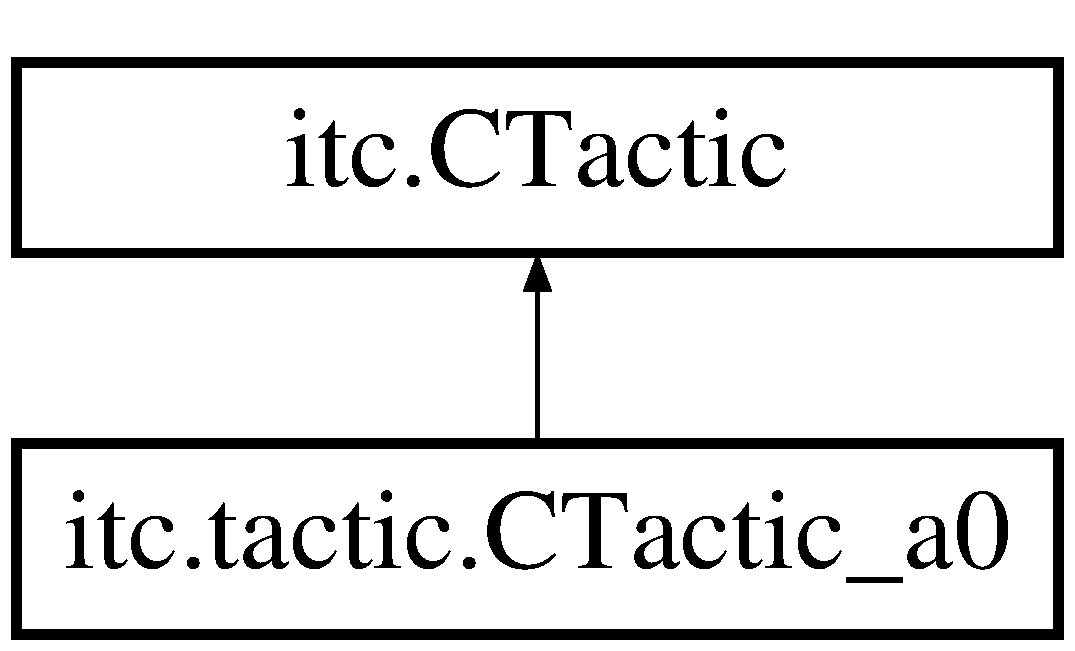
\includegraphics[height=2cm]{classitc_1_1tactic_1_1_c_tactic__a0}
\end{center}
\end{figure}
\subsection*{Public Member Functions}
\begin{DoxyCompactItemize}
\item 
void \hyperlink{classitc_1_1tactic_1_1_c_tactic__a0_a7d6f39924f332a7ed8c53820a45d3834}{run\_\-} (\hyperlink{classitc_1_1solomon}{solomon} s)
\item 
void \hyperlink{classitc_1_1tactic_1_1_c_tactic__a0_aea5ad2191ee16822a129eafb37d91779}{onScannedRobot\_\-} (\hyperlink{classitc_1_1solomon}{solomon} s, ScannedRobotEvent e)
\item 
void \hyperlink{classitc_1_1tactic_1_1_c_tactic__a0_a8911e3200cb13cfab22082c0a718c0b9}{onHitByBullet\_\-} (\hyperlink{classitc_1_1solomon}{solomon} s, HitByBulletEvent e)
\end{DoxyCompactItemize}


\subsection{Member Function Documentation}
\hypertarget{classitc_1_1tactic_1_1_c_tactic__a0_a8911e3200cb13cfab22082c0a718c0b9}{
\index{itc::tactic::CTactic\_\-a0@{itc::tactic::CTactic\_\-a0}!onHitByBullet\_\-@{onHitByBullet\_\-}}
\index{onHitByBullet\_\-@{onHitByBullet\_\-}!itc::tactic::CTactic_a0@{itc::tactic::CTactic\_\-a0}}
\subsubsection[{onHitByBullet\_\-}]{\setlength{\rightskip}{0pt plus 5cm}void itc.tactic.CTactic\_\-a0.onHitByBullet\_\- ({\bf solomon} {\em s}, \/  HitByBulletEvent {\em e})}}
\label{classitc_1_1tactic_1_1_c_tactic__a0_a8911e3200cb13cfab22082c0a718c0b9}
This should be overwritten by every tactic. 
\begin{DoxyParams}{Parameters}
\item[{\em s}]\item[{\em e}]\end{DoxyParams}


Reimplemented from \hyperlink{classitc_1_1_c_tactic_a9a8d125f826667459758f2767c3bd957}{itc.CTactic}.\hypertarget{classitc_1_1tactic_1_1_c_tactic__a0_aea5ad2191ee16822a129eafb37d91779}{
\index{itc::tactic::CTactic\_\-a0@{itc::tactic::CTactic\_\-a0}!onScannedRobot\_\-@{onScannedRobot\_\-}}
\index{onScannedRobot\_\-@{onScannedRobot\_\-}!itc::tactic::CTactic_a0@{itc::tactic::CTactic\_\-a0}}
\subsubsection[{onScannedRobot\_\-}]{\setlength{\rightskip}{0pt plus 5cm}void itc.tactic.CTactic\_\-a0.onScannedRobot\_\- ({\bf solomon} {\em s}, \/  ScannedRobotEvent {\em e})}}
\label{classitc_1_1tactic_1_1_c_tactic__a0_aea5ad2191ee16822a129eafb37d91779}
This should be overwritten by every tactic. 
\begin{DoxyParams}{Parameters}
\item[{\em s}]\item[{\em e}]\end{DoxyParams}


Reimplemented from \hyperlink{classitc_1_1_c_tactic_a63a5a64ff30293061e37eca71fb77a96}{itc.CTactic}.\hypertarget{classitc_1_1tactic_1_1_c_tactic__a0_a7d6f39924f332a7ed8c53820a45d3834}{
\index{itc::tactic::CTactic\_\-a0@{itc::tactic::CTactic\_\-a0}!run\_\-@{run\_\-}}
\index{run\_\-@{run\_\-}!itc::tactic::CTactic_a0@{itc::tactic::CTactic\_\-a0}}
\subsubsection[{run\_\-}]{\setlength{\rightskip}{0pt plus 5cm}void itc.tactic.CTactic\_\-a0.run\_\- ({\bf solomon} {\em s})}}
\label{classitc_1_1tactic_1_1_c_tactic__a0_a7d6f39924f332a7ed8c53820a45d3834}
This should be overwritten by every tactic. 
\begin{DoxyParams}{Parameters}
\item[{\em s}]\end{DoxyParams}


Reimplemented from \hyperlink{classitc_1_1_c_tactic_ae5f5c51a6e04d22bc298dbdec4080770}{itc.CTactic}.

The documentation for this class was generated from the following file:\begin{DoxyCompactItemize}
\item 
/Users/carllange/Documents/workspace/Solomon/src/itc/tactic/CTactic\_\-a0.java\end{DoxyCompactItemize}

\hypertarget{classitc_1_1tactic_1_1_c_tactic__a1}{
\section{itc.tactic.CTactic\_\-a1 Class Reference}
\label{classitc_1_1tactic_1_1_c_tactic__a1}\index{itc::tactic::CTactic\_\-a1@{itc::tactic::CTactic\_\-a1}}
}
Inheritance diagram for itc.tactic.CTactic\_\-a1::\begin{figure}[H]
\begin{center}
\leavevmode
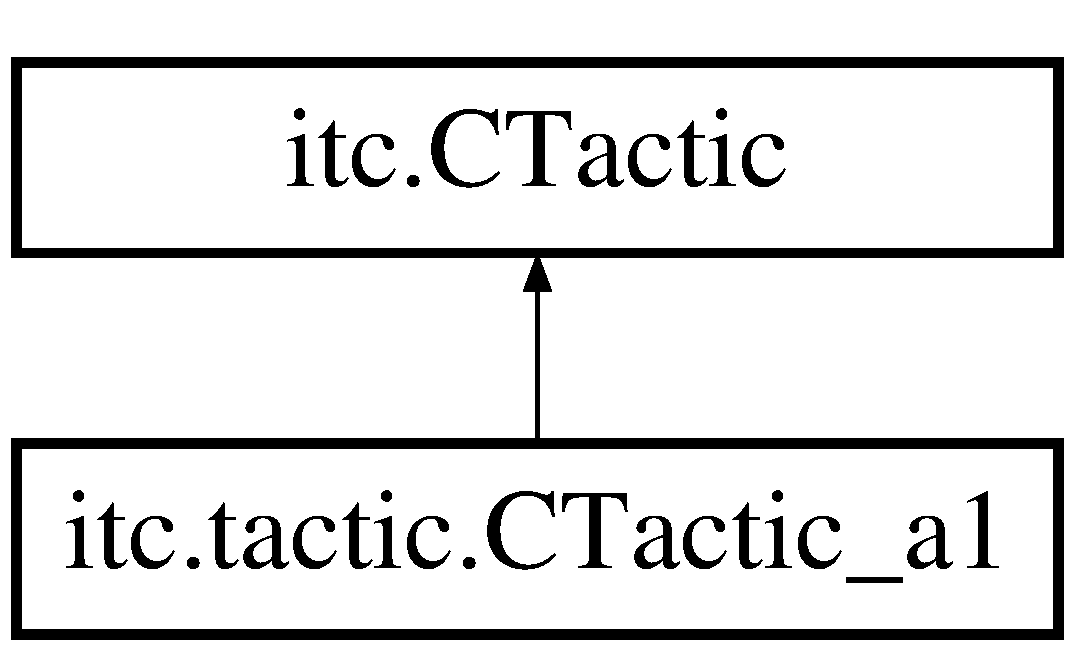
\includegraphics[height=2cm]{classitc_1_1tactic_1_1_c_tactic__a1}
\end{center}
\end{figure}
\subsection*{Public Member Functions}
\begin{DoxyCompactItemize}
\item 
void \hyperlink{classitc_1_1tactic_1_1_c_tactic__a1_a83dba0cef825a91cd2818e3246a77a76}{run\_\-} (\hyperlink{classitc_1_1solomon}{solomon} s)
\item 
void \hyperlink{classitc_1_1tactic_1_1_c_tactic__a1_aab5562fb9a1ed47924bdf4c1d6eb10de}{onScannedRobot\_\-} (\hyperlink{classitc_1_1solomon}{solomon} s, ScannedRobotEvent e)
\item 
void \hyperlink{classitc_1_1tactic_1_1_c_tactic__a1_ac61ce5dba31a140581a5f6f2dd74d73b}{onHitRobot\_\-} (\hyperlink{classitc_1_1solomon}{solomon} s, HitRobotEvent e)
\end{DoxyCompactItemize}


\subsection{Member Function Documentation}
\hypertarget{classitc_1_1tactic_1_1_c_tactic__a1_ac61ce5dba31a140581a5f6f2dd74d73b}{
\index{itc::tactic::CTactic\_\-a1@{itc::tactic::CTactic\_\-a1}!onHitRobot\_\-@{onHitRobot\_\-}}
\index{onHitRobot\_\-@{onHitRobot\_\-}!itc::tactic::CTactic_a1@{itc::tactic::CTactic\_\-a1}}
\subsubsection[{onHitRobot\_\-}]{\setlength{\rightskip}{0pt plus 5cm}void itc.tactic.CTactic\_\-a1.onHitRobot\_\- ({\bf solomon} {\em s}, \/  HitRobotEvent {\em e})}}
\label{classitc_1_1tactic_1_1_c_tactic__a1_ac61ce5dba31a140581a5f6f2dd74d73b}
onHitRobot: If it's our fault, we'll stop turning and moving, so we need to turn again to keep spinning. 

Reimplemented from \hyperlink{classitc_1_1_c_tactic_a19cf73207948eff2c6db7d90fce8bd55}{itc.CTactic}.\hypertarget{classitc_1_1tactic_1_1_c_tactic__a1_aab5562fb9a1ed47924bdf4c1d6eb10de}{
\index{itc::tactic::CTactic\_\-a1@{itc::tactic::CTactic\_\-a1}!onScannedRobot\_\-@{onScannedRobot\_\-}}
\index{onScannedRobot\_\-@{onScannedRobot\_\-}!itc::tactic::CTactic_a1@{itc::tactic::CTactic\_\-a1}}
\subsubsection[{onScannedRobot\_\-}]{\setlength{\rightskip}{0pt plus 5cm}void itc.tactic.CTactic\_\-a1.onScannedRobot\_\- ({\bf solomon} {\em s}, \/  ScannedRobotEvent {\em e})}}
\label{classitc_1_1tactic_1_1_c_tactic__a1_aab5562fb9a1ed47924bdf4c1d6eb10de}
This should be overwritten by every tactic. 
\begin{DoxyParams}{Parameters}
\item[{\em s}]\item[{\em e}]\end{DoxyParams}


Reimplemented from \hyperlink{classitc_1_1_c_tactic_a63a5a64ff30293061e37eca71fb77a96}{itc.CTactic}.\hypertarget{classitc_1_1tactic_1_1_c_tactic__a1_a83dba0cef825a91cd2818e3246a77a76}{
\index{itc::tactic::CTactic\_\-a1@{itc::tactic::CTactic\_\-a1}!run\_\-@{run\_\-}}
\index{run\_\-@{run\_\-}!itc::tactic::CTactic_a1@{itc::tactic::CTactic\_\-a1}}
\subsubsection[{run\_\-}]{\setlength{\rightskip}{0pt plus 5cm}void itc.tactic.CTactic\_\-a1.run\_\- ({\bf solomon} {\em s})}}
\label{classitc_1_1tactic_1_1_c_tactic__a1_a83dba0cef825a91cd2818e3246a77a76}
This should be overwritten by every tactic. 
\begin{DoxyParams}{Parameters}
\item[{\em s}]\end{DoxyParams}


Reimplemented from \hyperlink{classitc_1_1_c_tactic_ae5f5c51a6e04d22bc298dbdec4080770}{itc.CTactic}.

The documentation for this class was generated from the following file:\begin{DoxyCompactItemize}
\item 
/Users/carllange/Documents/workspace/Solomon/src/itc/tactic/CTactic\_\-a1.java\end{DoxyCompactItemize}

\hypertarget{classitc_1_1tactic_1_1_c_tactic__a2}{
\section{itc.tactic.CTactic\_\-a2 Class Reference}
\label{classitc_1_1tactic_1_1_c_tactic__a2}\index{itc::tactic::CTactic\_\-a2@{itc::tactic::CTactic\_\-a2}}
}
Inheritance diagram for itc.tactic.CTactic\_\-a2::\begin{figure}[H]
\begin{center}
\leavevmode
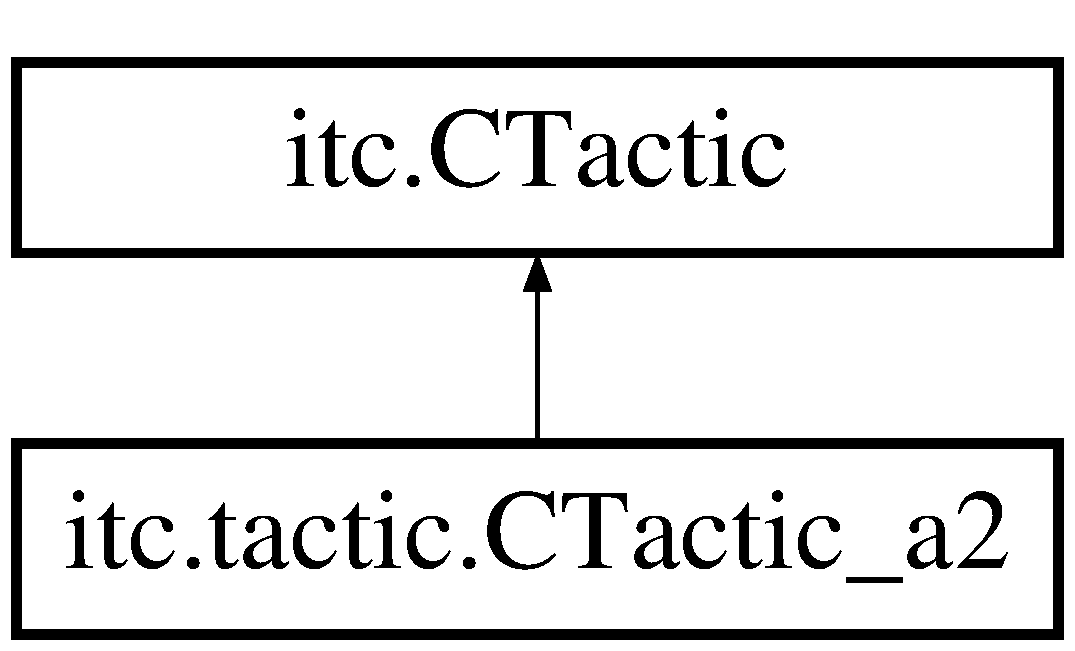
\includegraphics[height=2cm]{classitc_1_1tactic_1_1_c_tactic__a2}
\end{center}
\end{figure}
\subsection*{Public Member Functions}
\begin{DoxyCompactItemize}
\item 
void \hyperlink{classitc_1_1tactic_1_1_c_tactic__a2_a71e36f42565ca1436eb1ee71f3d94312}{run\_\-} (\hyperlink{classitc_1_1solomon}{solomon} s)
\item 
void \hyperlink{classitc_1_1tactic_1_1_c_tactic__a2_a2448157d91e699740cf8a99f99b0c456}{onScannedRobot\_\-} (\hyperlink{classitc_1_1solomon}{solomon} s, ScannedRobotEvent e)
\item 
void \hyperlink{classitc_1_1tactic_1_1_c_tactic__a2_a774862588c2b010b16e2709d922db24d}{onHitByBullet\_\-} (\hyperlink{classitc_1_1solomon}{solomon} s, HitByBulletEvent e)
\end{DoxyCompactItemize}


\subsection{Member Function Documentation}
\hypertarget{classitc_1_1tactic_1_1_c_tactic__a2_a774862588c2b010b16e2709d922db24d}{
\index{itc::tactic::CTactic\_\-a2@{itc::tactic::CTactic\_\-a2}!onHitByBullet\_\-@{onHitByBullet\_\-}}
\index{onHitByBullet\_\-@{onHitByBullet\_\-}!itc::tactic::CTactic_a2@{itc::tactic::CTactic\_\-a2}}
\subsubsection[{onHitByBullet\_\-}]{\setlength{\rightskip}{0pt plus 5cm}void itc.tactic.CTactic\_\-a2.onHitByBullet\_\- ({\bf solomon} {\em s}, \/  HitByBulletEvent {\em e})}}
\label{classitc_1_1tactic_1_1_c_tactic__a2_a774862588c2b010b16e2709d922db24d}
This should be overwritten by every tactic. 
\begin{DoxyParams}{Parameters}
\item[{\em s}]\item[{\em e}]\end{DoxyParams}


Reimplemented from \hyperlink{classitc_1_1_c_tactic_a9a8d125f826667459758f2767c3bd957}{itc.CTactic}.\hypertarget{classitc_1_1tactic_1_1_c_tactic__a2_a2448157d91e699740cf8a99f99b0c456}{
\index{itc::tactic::CTactic\_\-a2@{itc::tactic::CTactic\_\-a2}!onScannedRobot\_\-@{onScannedRobot\_\-}}
\index{onScannedRobot\_\-@{onScannedRobot\_\-}!itc::tactic::CTactic_a2@{itc::tactic::CTactic\_\-a2}}
\subsubsection[{onScannedRobot\_\-}]{\setlength{\rightskip}{0pt plus 5cm}void itc.tactic.CTactic\_\-a2.onScannedRobot\_\- ({\bf solomon} {\em s}, \/  ScannedRobotEvent {\em e})}}
\label{classitc_1_1tactic_1_1_c_tactic__a2_a2448157d91e699740cf8a99f99b0c456}
This should be overwritten by every tactic. 
\begin{DoxyParams}{Parameters}
\item[{\em s}]\item[{\em e}]\end{DoxyParams}


Reimplemented from \hyperlink{classitc_1_1_c_tactic_a63a5a64ff30293061e37eca71fb77a96}{itc.CTactic}.\hypertarget{classitc_1_1tactic_1_1_c_tactic__a2_a71e36f42565ca1436eb1ee71f3d94312}{
\index{itc::tactic::CTactic\_\-a2@{itc::tactic::CTactic\_\-a2}!run\_\-@{run\_\-}}
\index{run\_\-@{run\_\-}!itc::tactic::CTactic_a2@{itc::tactic::CTactic\_\-a2}}
\subsubsection[{run\_\-}]{\setlength{\rightskip}{0pt plus 5cm}void itc.tactic.CTactic\_\-a2.run\_\- ({\bf solomon} {\em s})}}
\label{classitc_1_1tactic_1_1_c_tactic__a2_a71e36f42565ca1436eb1ee71f3d94312}
This should be overwritten by every tactic. 
\begin{DoxyParams}{Parameters}
\item[{\em s}]\end{DoxyParams}


Reimplemented from \hyperlink{classitc_1_1_c_tactic_ae5f5c51a6e04d22bc298dbdec4080770}{itc.CTactic}.

The documentation for this class was generated from the following file:\begin{DoxyCompactItemize}
\item 
/Users/carllange/Documents/workspace/Solomon/src/itc/tactic/CTactic\_\-a2.java\end{DoxyCompactItemize}

\hypertarget{classitc_1_1tactic_1_1_c_tactic__d0}{
\section{itc.tactic.CTactic\_\-d0 Class Reference}
\label{classitc_1_1tactic_1_1_c_tactic__d0}\index{itc::tactic::CTactic\_\-d0@{itc::tactic::CTactic\_\-d0}}
}
Inheritance diagram for itc.tactic.CTactic\_\-d0::\begin{figure}[H]
\begin{center}
\leavevmode
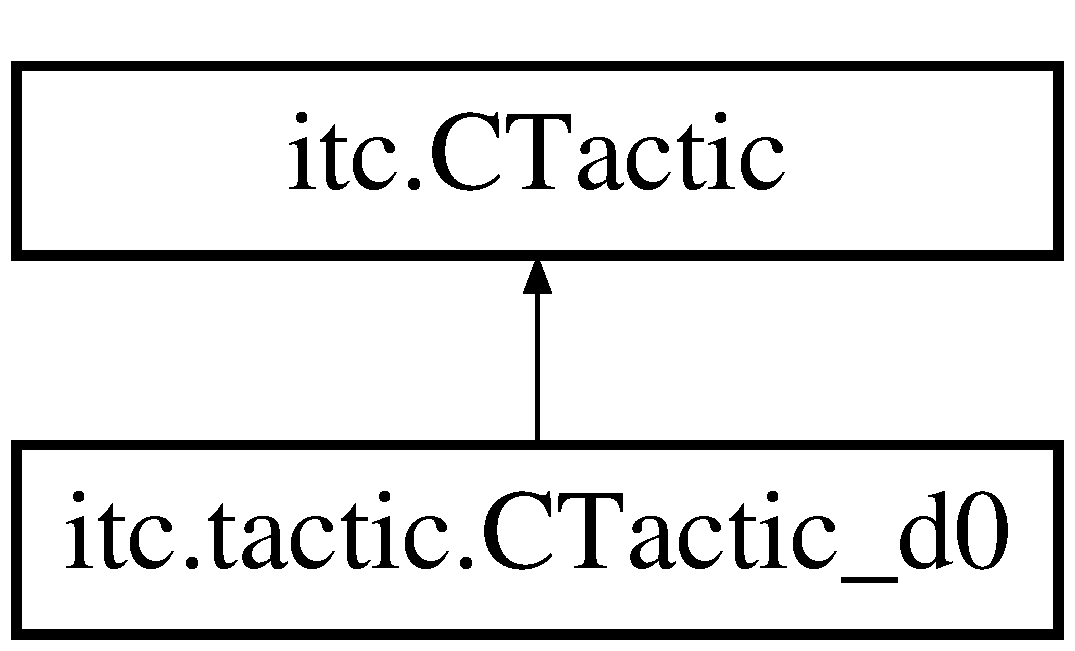
\includegraphics[height=2cm]{classitc_1_1tactic_1_1_c_tactic__d0}
\end{center}
\end{figure}
\subsection*{Public Member Functions}
\begin{DoxyCompactItemize}
\item 
void \hyperlink{classitc_1_1tactic_1_1_c_tactic__d0_a1f8e1863b6d1848867239230dd77b8f8}{run\_\-} (\hyperlink{classitc_1_1solomon}{solomon} s)
\item 
void \hyperlink{classitc_1_1tactic_1_1_c_tactic__d0_a85a50bae05c5e1b1bf7bdc450325ae0e}{onScannedRobot\_\-} (\hyperlink{classitc_1_1solomon}{solomon} s, ScannedRobotEvent e)
\item 
void \hyperlink{classitc_1_1tactic_1_1_c_tactic__d0_a4af101273ae2df9ee3c58641e1b1e422}{onHitByBullet\_\-} (\hyperlink{classitc_1_1solomon}{solomon} s, HitByBulletEvent e)
\end{DoxyCompactItemize}


\subsection{Detailed Description}
Defensive tactic.

\begin{DoxyAuthor}{Author}
Carl Lange 
\end{DoxyAuthor}


\subsection{Member Function Documentation}
\hypertarget{classitc_1_1tactic_1_1_c_tactic__d0_a4af101273ae2df9ee3c58641e1b1e422}{
\index{itc::tactic::CTactic\_\-d0@{itc::tactic::CTactic\_\-d0}!onHitByBullet\_\-@{onHitByBullet\_\-}}
\index{onHitByBullet\_\-@{onHitByBullet\_\-}!itc::tactic::CTactic_d0@{itc::tactic::CTactic\_\-d0}}
\subsubsection[{onHitByBullet\_\-}]{\setlength{\rightskip}{0pt plus 5cm}void itc.tactic.CTactic\_\-d0.onHitByBullet\_\- ({\bf solomon} {\em s}, \/  HitByBulletEvent {\em e})}}
\label{classitc_1_1tactic_1_1_c_tactic__d0_a4af101273ae2df9ee3c58641e1b1e422}
This should be overwritten by every tactic. 
\begin{DoxyParams}{Parameters}
\item[{\em s}]\item[{\em e}]\end{DoxyParams}


Reimplemented from \hyperlink{classitc_1_1_c_tactic_a9a8d125f826667459758f2767c3bd957}{itc.CTactic}.\hypertarget{classitc_1_1tactic_1_1_c_tactic__d0_a85a50bae05c5e1b1bf7bdc450325ae0e}{
\index{itc::tactic::CTactic\_\-d0@{itc::tactic::CTactic\_\-d0}!onScannedRobot\_\-@{onScannedRobot\_\-}}
\index{onScannedRobot\_\-@{onScannedRobot\_\-}!itc::tactic::CTactic_d0@{itc::tactic::CTactic\_\-d0}}
\subsubsection[{onScannedRobot\_\-}]{\setlength{\rightskip}{0pt plus 5cm}void itc.tactic.CTactic\_\-d0.onScannedRobot\_\- ({\bf solomon} {\em s}, \/  ScannedRobotEvent {\em e})}}
\label{classitc_1_1tactic_1_1_c_tactic__d0_a85a50bae05c5e1b1bf7bdc450325ae0e}
This should be overwritten by every tactic. 
\begin{DoxyParams}{Parameters}
\item[{\em s}]\item[{\em e}]\end{DoxyParams}


Reimplemented from \hyperlink{classitc_1_1_c_tactic_a63a5a64ff30293061e37eca71fb77a96}{itc.CTactic}.\hypertarget{classitc_1_1tactic_1_1_c_tactic__d0_a1f8e1863b6d1848867239230dd77b8f8}{
\index{itc::tactic::CTactic\_\-d0@{itc::tactic::CTactic\_\-d0}!run\_\-@{run\_\-}}
\index{run\_\-@{run\_\-}!itc::tactic::CTactic_d0@{itc::tactic::CTactic\_\-d0}}
\subsubsection[{run\_\-}]{\setlength{\rightskip}{0pt plus 5cm}void itc.tactic.CTactic\_\-d0.run\_\- ({\bf solomon} {\em s})}}
\label{classitc_1_1tactic_1_1_c_tactic__d0_a1f8e1863b6d1848867239230dd77b8f8}
This should be overwritten by every tactic. 
\begin{DoxyParams}{Parameters}
\item[{\em s}]\end{DoxyParams}


Reimplemented from \hyperlink{classitc_1_1_c_tactic_ae5f5c51a6e04d22bc298dbdec4080770}{itc.CTactic}.

The documentation for this class was generated from the following file:\begin{DoxyCompactItemize}
\item 
/Users/carllange/Documents/workspace/Solomon/src/itc/tactic/CTactic\_\-d0.java\end{DoxyCompactItemize}

\hypertarget{classitc_1_1tactic_1_1_c_tactic__ea0}{
\section{itc.tactic.CTactic\_\-ea0 Class Reference}
\label{classitc_1_1tactic_1_1_c_tactic__ea0}\index{itc::tactic::CTactic\_\-ea0@{itc::tactic::CTactic\_\-ea0}}
}
Inheritance diagram for itc.tactic.CTactic\_\-ea0::\begin{figure}[H]
\begin{center}
\leavevmode
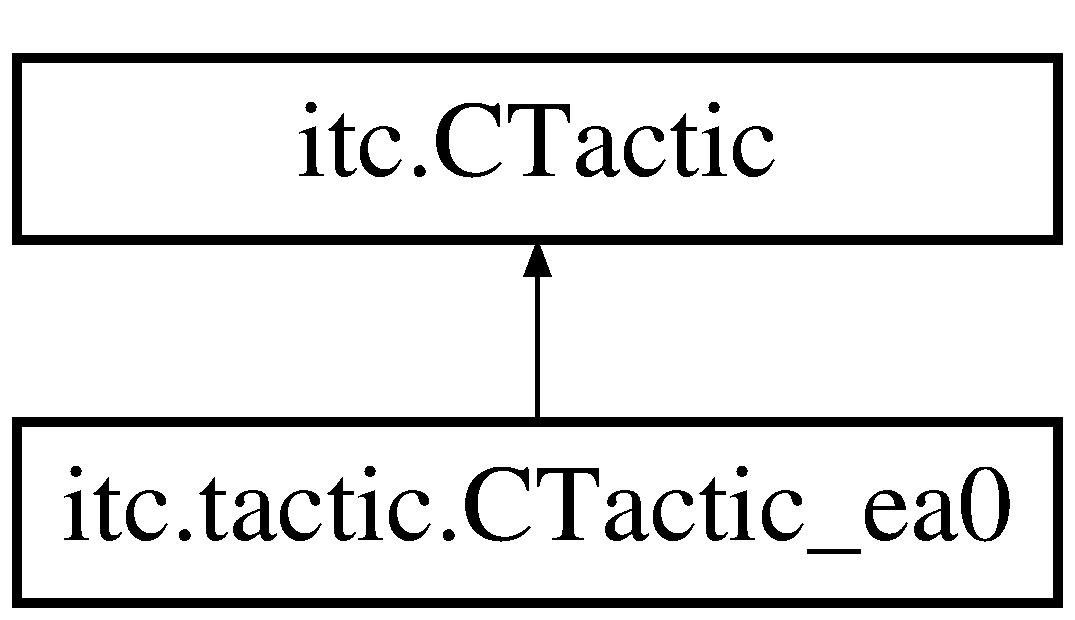
\includegraphics[height=2cm]{classitc_1_1tactic_1_1_c_tactic__ea0}
\end{center}
\end{figure}
\subsection*{Public Member Functions}
\begin{DoxyCompactItemize}
\item 
void \hyperlink{classitc_1_1tactic_1_1_c_tactic__ea0_af5b367f093ebea65ef06b41b03432289}{run\_\-} (\hyperlink{classitc_1_1solomon}{solomon} s)
\item 
void \hyperlink{classitc_1_1tactic_1_1_c_tactic__ea0_a64e0ac47db137d34d3c52abbde65917f}{onScannedRobot\_\-} (\hyperlink{classitc_1_1solomon}{solomon} s, ScannedRobotEvent e)
\item 
void \hyperlink{classitc_1_1tactic_1_1_c_tactic__ea0_a66859754a34c07f83a114509a86914cb}{onHitByBullet\_\-} (\hyperlink{classitc_1_1solomon}{solomon} s, HitByBulletEvent e)
\end{DoxyCompactItemize}


\subsection{Detailed Description}
Moves as close as possible, firing as it retreats. Implements linear targeting and bullet strength modulation.

Some open-\/source code used for linear targeting implementation.

\begin{DoxyAuthor}{Author}
Carl Lange 
\end{DoxyAuthor}


\subsection{Member Function Documentation}
\hypertarget{classitc_1_1tactic_1_1_c_tactic__ea0_a66859754a34c07f83a114509a86914cb}{
\index{itc::tactic::CTactic\_\-ea0@{itc::tactic::CTactic\_\-ea0}!onHitByBullet\_\-@{onHitByBullet\_\-}}
\index{onHitByBullet\_\-@{onHitByBullet\_\-}!itc::tactic::CTactic_ea0@{itc::tactic::CTactic\_\-ea0}}
\subsubsection[{onHitByBullet\_\-}]{\setlength{\rightskip}{0pt plus 5cm}void itc.tactic.CTactic\_\-ea0.onHitByBullet\_\- ({\bf solomon} {\em s}, \/  HitByBulletEvent {\em e})}}
\label{classitc_1_1tactic_1_1_c_tactic__ea0_a66859754a34c07f83a114509a86914cb}
This should be overwritten by every tactic. 
\begin{DoxyParams}{Parameters}
\item[{\em s}]\item[{\em e}]\end{DoxyParams}


Reimplemented from \hyperlink{classitc_1_1_c_tactic_a9a8d125f826667459758f2767c3bd957}{itc.CTactic}.\hypertarget{classitc_1_1tactic_1_1_c_tactic__ea0_a64e0ac47db137d34d3c52abbde65917f}{
\index{itc::tactic::CTactic\_\-ea0@{itc::tactic::CTactic\_\-ea0}!onScannedRobot\_\-@{onScannedRobot\_\-}}
\index{onScannedRobot\_\-@{onScannedRobot\_\-}!itc::tactic::CTactic_ea0@{itc::tactic::CTactic\_\-ea0}}
\subsubsection[{onScannedRobot\_\-}]{\setlength{\rightskip}{0pt plus 5cm}void itc.tactic.CTactic\_\-ea0.onScannedRobot\_\- ({\bf solomon} {\em s}, \/  ScannedRobotEvent {\em e})}}
\label{classitc_1_1tactic_1_1_c_tactic__ea0_a64e0ac47db137d34d3c52abbde65917f}
This should be overwritten by every tactic. 
\begin{DoxyParams}{Parameters}
\item[{\em s}]\item[{\em e}]\end{DoxyParams}


Reimplemented from \hyperlink{classitc_1_1_c_tactic_a63a5a64ff30293061e37eca71fb77a96}{itc.CTactic}.\hypertarget{classitc_1_1tactic_1_1_c_tactic__ea0_af5b367f093ebea65ef06b41b03432289}{
\index{itc::tactic::CTactic\_\-ea0@{itc::tactic::CTactic\_\-ea0}!run\_\-@{run\_\-}}
\index{run\_\-@{run\_\-}!itc::tactic::CTactic_ea0@{itc::tactic::CTactic\_\-ea0}}
\subsubsection[{run\_\-}]{\setlength{\rightskip}{0pt plus 5cm}void itc.tactic.CTactic\_\-ea0.run\_\- ({\bf solomon} {\em s})}}
\label{classitc_1_1tactic_1_1_c_tactic__ea0_af5b367f093ebea65ef06b41b03432289}
This should be overwritten by every tactic. 
\begin{DoxyParams}{Parameters}
\item[{\em s}]\end{DoxyParams}


Reimplemented from \hyperlink{classitc_1_1_c_tactic_ae5f5c51a6e04d22bc298dbdec4080770}{itc.CTactic}.

The documentation for this class was generated from the following file:\begin{DoxyCompactItemize}
\item 
/Users/carllange/Documents/workspace/Solomon/src/itc/tactic/CTactic\_\-ea0.java\end{DoxyCompactItemize}

\hypertarget{classitc_1_1tactic_1_1_c_tactic__ea1}{
\section{itc.tactic.CTactic\_\-ea1 Class Reference}
\label{classitc_1_1tactic_1_1_c_tactic__ea1}\index{itc::tactic::CTactic\_\-ea1@{itc::tactic::CTactic\_\-ea1}}
}
Inheritance diagram for itc.tactic.CTactic\_\-ea1::\begin{figure}[H]
\begin{center}
\leavevmode
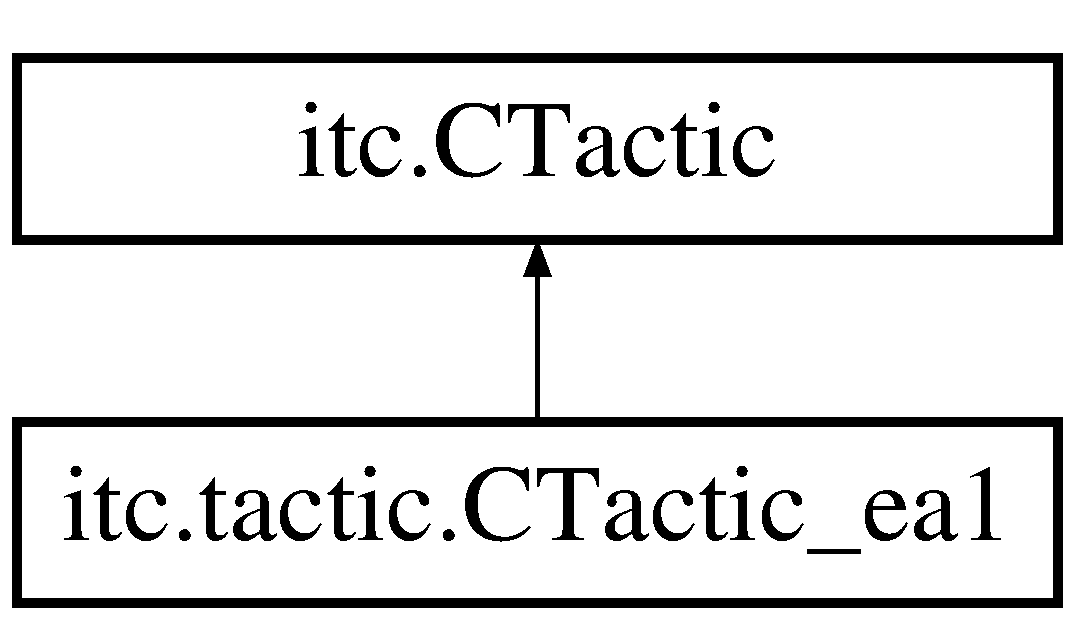
\includegraphics[height=2cm]{classitc_1_1tactic_1_1_c_tactic__ea1}
\end{center}
\end{figure}
\subsection*{Public Member Functions}
\begin{DoxyCompactItemize}
\item 
void \hyperlink{classitc_1_1tactic_1_1_c_tactic__ea1_ad3c677f7d3fbb5b88ebac50cd465a3cf}{run\_\-} (\hyperlink{classitc_1_1solomon}{solomon} s)
\item 
void \hyperlink{classitc_1_1tactic_1_1_c_tactic__ea1_aa483435460b0ee4fabe62e2d46493c7d}{onScannedRobot\_\-} (\hyperlink{classitc_1_1solomon}{solomon} s, ScannedRobotEvent e)
\item 
void \hyperlink{classitc_1_1tactic_1_1_c_tactic__ea1_a2eb8e76f5f9f629359436a611b8a09e5}{onHitRobot\_\-} (\hyperlink{classitc_1_1solomon}{solomon} s, HitRobotEvent e)
\item 
void \hyperlink{classitc_1_1tactic_1_1_c_tactic__ea1_a796f0c1b21f72300fbbd7cbccc6ef610}{onWin} (\hyperlink{classitc_1_1solomon}{solomon} s, WinEvent e)
\item 
double \hyperlink{classitc_1_1tactic_1_1_c_tactic__ea1_a3b4e695a085e2c955ec3059059df5eb5}{normalAbsoluteAngle} (double angle)
\item 
double \hyperlink{classitc_1_1tactic_1_1_c_tactic__ea1_ad3ae664f65b129510e03e04b83ad2fc2}{normalRelativeAngle} (double angle)
\end{DoxyCompactItemize}
\subsection*{Package Attributes}
\begin{DoxyCompactItemize}
\item 
\hypertarget{classitc_1_1tactic_1_1_c_tactic__ea1_aebc2e4dfb0db7531206e2aa78d3497a0}{
int {\bfseries count} = 0}
\label{classitc_1_1tactic_1_1_c_tactic__ea1_aebc2e4dfb0db7531206e2aa78d3497a0}

\item 
\hypertarget{classitc_1_1tactic_1_1_c_tactic__ea1_ae05b4d6d78518d268d58bfb3c76a2262}{
double {\bfseries gunTurnAmt}}
\label{classitc_1_1tactic_1_1_c_tactic__ea1_ae05b4d6d78518d268d58bfb3c76a2262}

\item 
\hypertarget{classitc_1_1tactic_1_1_c_tactic__ea1_afac095ae1f854bc0466df99f7a646d28}{
String {\bfseries trackName}}
\label{classitc_1_1tactic_1_1_c_tactic__ea1_afac095ae1f854bc0466df99f7a646d28}

\end{DoxyCompactItemize}


\subsection{Member Function Documentation}
\hypertarget{classitc_1_1tactic_1_1_c_tactic__ea1_a3b4e695a085e2c955ec3059059df5eb5}{
\index{itc::tactic::CTactic\_\-ea1@{itc::tactic::CTactic\_\-ea1}!normalAbsoluteAngle@{normalAbsoluteAngle}}
\index{normalAbsoluteAngle@{normalAbsoluteAngle}!itc::tactic::CTactic_ea1@{itc::tactic::CTactic\_\-ea1}}
\subsubsection[{normalAbsoluteAngle}]{\setlength{\rightskip}{0pt plus 5cm}double itc.tactic.CTactic\_\-ea1.normalAbsoluteAngle (double {\em angle})}}
\label{classitc_1_1tactic_1_1_c_tactic__ea1_a3b4e695a085e2c955ec3059059df5eb5}
normalAbsoluteAngle: Returns angle such that 0 $<$= angle $<$ 360 \hypertarget{classitc_1_1tactic_1_1_c_tactic__ea1_ad3ae664f65b129510e03e04b83ad2fc2}{
\index{itc::tactic::CTactic\_\-ea1@{itc::tactic::CTactic\_\-ea1}!normalRelativeAngle@{normalRelativeAngle}}
\index{normalRelativeAngle@{normalRelativeAngle}!itc::tactic::CTactic_ea1@{itc::tactic::CTactic\_\-ea1}}
\subsubsection[{normalRelativeAngle}]{\setlength{\rightskip}{0pt plus 5cm}double itc.tactic.CTactic\_\-ea1.normalRelativeAngle (double {\em angle})}}
\label{classitc_1_1tactic_1_1_c_tactic__ea1_ad3ae664f65b129510e03e04b83ad2fc2}
normalRelativeAngle: Returns angle such that -\/180 $<$ angle $<$= 180 \hypertarget{classitc_1_1tactic_1_1_c_tactic__ea1_a2eb8e76f5f9f629359436a611b8a09e5}{
\index{itc::tactic::CTactic\_\-ea1@{itc::tactic::CTactic\_\-ea1}!onHitRobot\_\-@{onHitRobot\_\-}}
\index{onHitRobot\_\-@{onHitRobot\_\-}!itc::tactic::CTactic_ea1@{itc::tactic::CTactic\_\-ea1}}
\subsubsection[{onHitRobot\_\-}]{\setlength{\rightskip}{0pt plus 5cm}void itc.tactic.CTactic\_\-ea1.onHitRobot\_\- ({\bf solomon} {\em s}, \/  HitRobotEvent {\em e})}}
\label{classitc_1_1tactic_1_1_c_tactic__ea1_a2eb8e76f5f9f629359436a611b8a09e5}
onHitRobot: Set him as our new target 

Reimplemented from \hyperlink{classitc_1_1_c_tactic_a19cf73207948eff2c6db7d90fce8bd55}{itc.CTactic}.\hypertarget{classitc_1_1tactic_1_1_c_tactic__ea1_aa483435460b0ee4fabe62e2d46493c7d}{
\index{itc::tactic::CTactic\_\-ea1@{itc::tactic::CTactic\_\-ea1}!onScannedRobot\_\-@{onScannedRobot\_\-}}
\index{onScannedRobot\_\-@{onScannedRobot\_\-}!itc::tactic::CTactic_ea1@{itc::tactic::CTactic\_\-ea1}}
\subsubsection[{onScannedRobot\_\-}]{\setlength{\rightskip}{0pt plus 5cm}void itc.tactic.CTactic\_\-ea1.onScannedRobot\_\- ({\bf solomon} {\em s}, \/  ScannedRobotEvent {\em e})}}
\label{classitc_1_1tactic_1_1_c_tactic__ea1_aa483435460b0ee4fabe62e2d46493c7d}
onScannedRobot: Here's the good stuff 

Reimplemented from \hyperlink{classitc_1_1_c_tactic_a63a5a64ff30293061e37eca71fb77a96}{itc.CTactic}.\hypertarget{classitc_1_1tactic_1_1_c_tactic__ea1_a796f0c1b21f72300fbbd7cbccc6ef610}{
\index{itc::tactic::CTactic\_\-ea1@{itc::tactic::CTactic\_\-ea1}!onWin@{onWin}}
\index{onWin@{onWin}!itc::tactic::CTactic_ea1@{itc::tactic::CTactic\_\-ea1}}
\subsubsection[{onWin}]{\setlength{\rightskip}{0pt plus 5cm}void itc.tactic.CTactic\_\-ea1.onWin ({\bf solomon} {\em s}, \/  WinEvent {\em e})}}
\label{classitc_1_1tactic_1_1_c_tactic__ea1_a796f0c1b21f72300fbbd7cbccc6ef610}
onWin: Do a victory dance \hypertarget{classitc_1_1tactic_1_1_c_tactic__ea1_ad3c677f7d3fbb5b88ebac50cd465a3cf}{
\index{itc::tactic::CTactic\_\-ea1@{itc::tactic::CTactic\_\-ea1}!run\_\-@{run\_\-}}
\index{run\_\-@{run\_\-}!itc::tactic::CTactic_ea1@{itc::tactic::CTactic\_\-ea1}}
\subsubsection[{run\_\-}]{\setlength{\rightskip}{0pt plus 5cm}void itc.tactic.CTactic\_\-ea1.run\_\- ({\bf solomon} {\em s})}}
\label{classitc_1_1tactic_1_1_c_tactic__ea1_ad3c677f7d3fbb5b88ebac50cd465a3cf}
run: Tracker's main run function 

Reimplemented from \hyperlink{classitc_1_1_c_tactic_ae5f5c51a6e04d22bc298dbdec4080770}{itc.CTactic}.

The documentation for this class was generated from the following file:\begin{DoxyCompactItemize}
\item 
/Users/carllange/Documents/workspace/Solomon/src/itc/tactic/CTactic\_\-ea1.java\end{DoxyCompactItemize}

\hypertarget{classitc_1_1tactic_1_1_c_tactic__ed0}{
\section{itc.tactic.CTactic\_\-ed0 Class Reference}
\label{classitc_1_1tactic_1_1_c_tactic__ed0}\index{itc::tactic::CTactic\_\-ed0@{itc::tactic::CTactic\_\-ed0}}
}
Inheritance diagram for itc.tactic.CTactic\_\-ed0::\begin{figure}[H]
\begin{center}
\leavevmode
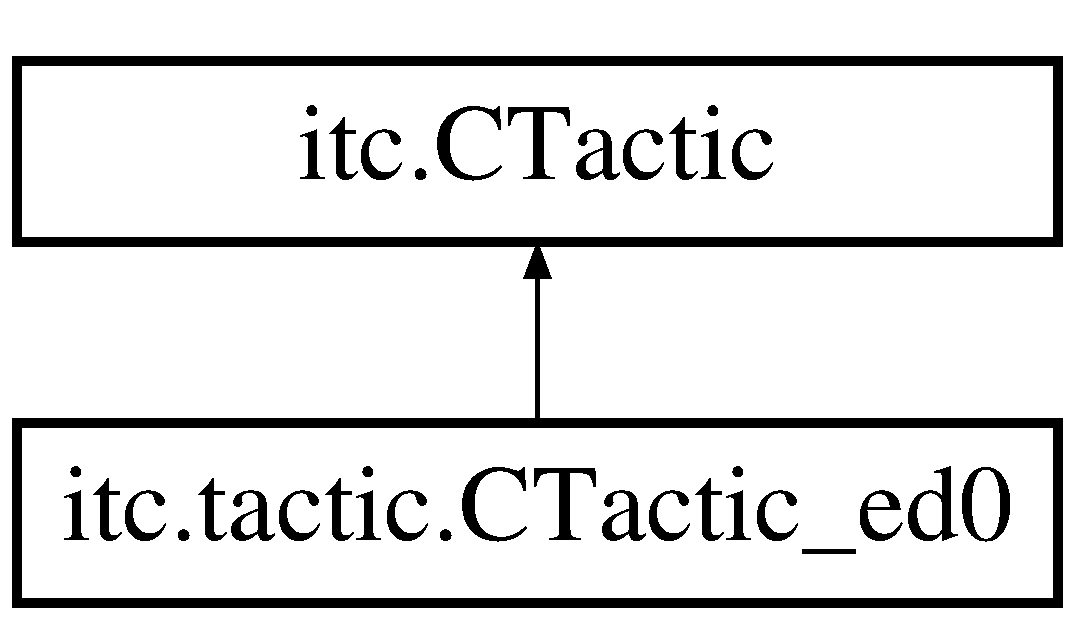
\includegraphics[height=2cm]{classitc_1_1tactic_1_1_c_tactic__ed0}
\end{center}
\end{figure}
\subsection*{Public Member Functions}
\begin{DoxyCompactItemize}
\item 
void \hyperlink{classitc_1_1tactic_1_1_c_tactic__ed0_aa8db38d3d879327bb337138a8f42a069}{run\_\-} (\hyperlink{classitc_1_1solomon}{solomon} s)
\item 
void \hyperlink{classitc_1_1tactic_1_1_c_tactic__ed0_aa1b6857853a2bc90fcf4309b39a3907a}{onScannedRobot\_\-} (\hyperlink{classitc_1_1solomon}{solomon} s, ScannedRobotEvent e)
\item 
void \hyperlink{classitc_1_1tactic_1_1_c_tactic__ed0_ad04cdcbec1998d1c7bee55a9dc959505}{onHitByBullet\_\-} (\hyperlink{classitc_1_1solomon}{solomon} s, HitByBulletEvent e)
\end{DoxyCompactItemize}
\subsection*{Package Attributes}
\begin{DoxyCompactItemize}
\item 
\hypertarget{classitc_1_1tactic_1_1_c_tactic__ed0_a34362d0142747b753729bfe67ae9b7e9}{
boolean {\bfseries scannedRobotYet} = false}
\label{classitc_1_1tactic_1_1_c_tactic__ed0_a34362d0142747b753729bfe67ae9b7e9}

\item 
\hypertarget{classitc_1_1tactic_1_1_c_tactic__ed0_aa35faecdb387aa9b98ff7ee2177919c0}{
double {\bfseries enemyDistance} = -\/1}
\label{classitc_1_1tactic_1_1_c_tactic__ed0_aa35faecdb387aa9b98ff7ee2177919c0}

\item 
\hypertarget{classitc_1_1tactic_1_1_c_tactic__ed0_ad16009212997fe1ba06e045c97483920}{
double {\bfseries furthestPossibleDistance} = -\/1}
\label{classitc_1_1tactic_1_1_c_tactic__ed0_ad16009212997fe1ba06e045c97483920}

\end{DoxyCompactItemize}


\subsection{Detailed Description}
This needs documentation and better commenting. TODO: Make this better, damnit. \begin{DoxyAuthor}{Author}
carllange 
\end{DoxyAuthor}


\subsection{Member Function Documentation}
\hypertarget{classitc_1_1tactic_1_1_c_tactic__ed0_ad04cdcbec1998d1c7bee55a9dc959505}{
\index{itc::tactic::CTactic\_\-ed0@{itc::tactic::CTactic\_\-ed0}!onHitByBullet\_\-@{onHitByBullet\_\-}}
\index{onHitByBullet\_\-@{onHitByBullet\_\-}!itc::tactic::CTactic_ed0@{itc::tactic::CTactic\_\-ed0}}
\subsubsection[{onHitByBullet\_\-}]{\setlength{\rightskip}{0pt plus 5cm}void itc.tactic.CTactic\_\-ed0.onHitByBullet\_\- ({\bf solomon} {\em s}, \/  HitByBulletEvent {\em e})}}
\label{classitc_1_1tactic_1_1_c_tactic__ed0_ad04cdcbec1998d1c7bee55a9dc959505}
This should be overwritten by every tactic. 
\begin{DoxyParams}{Parameters}
\item[{\em s}]\item[{\em e}]\end{DoxyParams}


Reimplemented from \hyperlink{classitc_1_1_c_tactic_a9a8d125f826667459758f2767c3bd957}{itc.CTactic}.\hypertarget{classitc_1_1tactic_1_1_c_tactic__ed0_aa1b6857853a2bc90fcf4309b39a3907a}{
\index{itc::tactic::CTactic\_\-ed0@{itc::tactic::CTactic\_\-ed0}!onScannedRobot\_\-@{onScannedRobot\_\-}}
\index{onScannedRobot\_\-@{onScannedRobot\_\-}!itc::tactic::CTactic_ed0@{itc::tactic::CTactic\_\-ed0}}
\subsubsection[{onScannedRobot\_\-}]{\setlength{\rightskip}{0pt plus 5cm}void itc.tactic.CTactic\_\-ed0.onScannedRobot\_\- ({\bf solomon} {\em s}, \/  ScannedRobotEvent {\em e})}}
\label{classitc_1_1tactic_1_1_c_tactic__ed0_aa1b6857853a2bc90fcf4309b39a3907a}
This should be overwritten by every tactic. 
\begin{DoxyParams}{Parameters}
\item[{\em s}]\item[{\em e}]\end{DoxyParams}


Reimplemented from \hyperlink{classitc_1_1_c_tactic_a63a5a64ff30293061e37eca71fb77a96}{itc.CTactic}.\hypertarget{classitc_1_1tactic_1_1_c_tactic__ed0_aa8db38d3d879327bb337138a8f42a069}{
\index{itc::tactic::CTactic\_\-ed0@{itc::tactic::CTactic\_\-ed0}!run\_\-@{run\_\-}}
\index{run\_\-@{run\_\-}!itc::tactic::CTactic_ed0@{itc::tactic::CTactic\_\-ed0}}
\subsubsection[{run\_\-}]{\setlength{\rightskip}{0pt plus 5cm}void itc.tactic.CTactic\_\-ed0.run\_\- ({\bf solomon} {\em s})}}
\label{classitc_1_1tactic_1_1_c_tactic__ed0_aa8db38d3d879327bb337138a8f42a069}
This should be overwritten by every tactic. 
\begin{DoxyParams}{Parameters}
\item[{\em s}]\end{DoxyParams}


Reimplemented from \hyperlink{classitc_1_1_c_tactic_ae5f5c51a6e04d22bc298dbdec4080770}{itc.CTactic}.

The documentation for this class was generated from the following file:\begin{DoxyCompactItemize}
\item 
/Users/carllange/Documents/workspace/Solomon/src/itc/tactic/CTactic\_\-ed0.java\end{DoxyCompactItemize}

\hypertarget{classitc_1_1solomon}{
\section{itc.solomon Class Reference}
\label{classitc_1_1solomon}\index{itc::solomon@{itc::solomon}}
}
\subsection*{Public Member Functions}
\begin{DoxyCompactItemize}
\item 
byte \hyperlink{classitc_1_1solomon_a1192c7e80d463fb5e0c6e5fc7f8b8944}{getStatus} ()
\item 
void \hyperlink{classitc_1_1solomon_aa16db4d650d1549fd1ae6426af16ea43}{setStatus} (byte status)
\item 
\hyperlink{classitc_1_1solomon_a774791cdf521fc7dc2118a761ccc0681}{solomon} ()
\item 
void \hyperlink{classitc_1_1solomon_a34ceb1ef78c0b0af58b074935e011a72}{run} ()
\item 
void \hyperlink{classitc_1_1solomon_a7b4f3c0da153c43da17a76c433770419}{onScannedRobot} (ScannedRobotEvent e)
\item 
void \hyperlink{classitc_1_1solomon_a61c2a71738163bea55b22c2ddd725117}{onHitByBullet} (HitByBulletEvent e)
\item 
void \hyperlink{classitc_1_1solomon_a5e824f07f03d305450e42a4356a003a5}{onHitRobot} (HitRobotEvent e)
\end{DoxyCompactItemize}
\subsection*{Package Attributes}
\begin{DoxyCompactItemize}
\item 
\hypertarget{classitc_1_1solomon_a6bea1eb6237528e23c4c4341e261c6ba}{
long {\bfseries maxduration} = 900}
\label{classitc_1_1solomon_a6bea1eb6237528e23c4c4341e261c6ba}

\item 
\hypertarget{classitc_1_1solomon_a2584be2758541c9758f9f3ba4ba06f42}{
long {\bfseries endtime} = 0}
\label{classitc_1_1solomon_a2584be2758541c9758f9f3ba4ba06f42}

\end{DoxyCompactItemize}


\subsection{Detailed Description}
Solomon -\/ a robot by IT Carlow students Ciaran McCann and Carl Lange. 

\subsection{Constructor \& Destructor Documentation}
\hypertarget{classitc_1_1solomon_a774791cdf521fc7dc2118a761ccc0681}{
\index{itc::solomon@{itc::solomon}!solomon@{solomon}}
\index{solomon@{solomon}!itc::solomon@{itc::solomon}}
\subsubsection[{solomon}]{\setlength{\rightskip}{0pt plus 5cm}itc.solomon.solomon ()}}
\label{classitc_1_1solomon_a774791cdf521fc7dc2118a761ccc0681}
The constructor for Solomon. Calls populateLibrary. 

\subsection{Member Function Documentation}
\hypertarget{classitc_1_1solomon_a1192c7e80d463fb5e0c6e5fc7f8b8944}{
\index{itc::solomon@{itc::solomon}!getStatus@{getStatus}}
\index{getStatus@{getStatus}!itc::solomon@{itc::solomon}}
\subsubsection[{getStatus}]{\setlength{\rightskip}{0pt plus 5cm}byte itc.solomon.getStatus ()}}
\label{classitc_1_1solomon_a1192c7e80d463fb5e0c6e5fc7f8b8944}
Simply returns the current status (0,1,2,3). \begin{DoxyReturn}{Returns}
currentStatus. 
\end{DoxyReturn}
\hypertarget{classitc_1_1solomon_a61c2a71738163bea55b22c2ddd725117}{
\index{itc::solomon@{itc::solomon}!onHitByBullet@{onHitByBullet}}
\index{onHitByBullet@{onHitByBullet}!itc::solomon@{itc::solomon}}
\subsubsection[{onHitByBullet}]{\setlength{\rightskip}{0pt plus 5cm}void itc.solomon.onHitByBullet (HitByBulletEvent {\em e})}}
\label{classitc_1_1solomon_a61c2a71738163bea55b22c2ddd725117}
onHitByBullet: What to do when you're hit by a bullet. This calls the current tactic's onHitByBullet\_\-() method. \hypertarget{classitc_1_1solomon_a5e824f07f03d305450e42a4356a003a5}{
\index{itc::solomon@{itc::solomon}!onHitRobot@{onHitRobot}}
\index{onHitRobot@{onHitRobot}!itc::solomon@{itc::solomon}}
\subsubsection[{onHitRobot}]{\setlength{\rightskip}{0pt plus 5cm}void itc.solomon.onHitRobot (HitRobotEvent {\em e})}}
\label{classitc_1_1solomon_a5e824f07f03d305450e42a4356a003a5}
onHitRobot: What to do when you hit another robot. This calls the current tactic's onHitRobot\_\-() method. \hypertarget{classitc_1_1solomon_a7b4f3c0da153c43da17a76c433770419}{
\index{itc::solomon@{itc::solomon}!onScannedRobot@{onScannedRobot}}
\index{onScannedRobot@{onScannedRobot}!itc::solomon@{itc::solomon}}
\subsubsection[{onScannedRobot}]{\setlength{\rightskip}{0pt plus 5cm}void itc.solomon.onScannedRobot (ScannedRobotEvent {\em e})}}
\label{classitc_1_1solomon_a7b4f3c0da153c43da17a76c433770419}
onScannedRobot: What to do when you see another robot. This calls the current tactic's onScannedRobot\_\-() method. \hypertarget{classitc_1_1solomon_a34ceb1ef78c0b0af58b074935e011a72}{
\index{itc::solomon@{itc::solomon}!run@{run}}
\index{run@{run}!itc::solomon@{itc::solomon}}
\subsubsection[{run}]{\setlength{\rightskip}{0pt plus 5cm}void itc.solomon.run ()}}
\label{classitc_1_1solomon_a34ceb1ef78c0b0af58b074935e011a72}
This sets Solomon's colours, then goes into an infinite loop. This loop is Solomon's main loop (its \char`\"{}game loop\char`\"{}, of sorts. \hypertarget{classitc_1_1solomon_aa16db4d650d1549fd1ae6426af16ea43}{
\index{itc::solomon@{itc::solomon}!setStatus@{setStatus}}
\index{setStatus@{setStatus}!itc::solomon@{itc::solomon}}
\subsubsection[{setStatus}]{\setlength{\rightskip}{0pt plus 5cm}void itc.solomon.setStatus (byte {\em status})}}
\label{classitc_1_1solomon_aa16db4d650d1549fd1ae6426af16ea43}
Simply sets the current status (0,1,2,3). 
\begin{DoxyParams}{Parameters}
\item[{\em status}]\end{DoxyParams}


The documentation for this class was generated from the following file:\begin{DoxyCompactItemize}
\item 
/Users/carllange/Documents/workspace/Solomon/src/itc/solomon.java\end{DoxyCompactItemize}

\printindex
\end{document}
